% CENG 467 term-project presentation
% Build: latexmk -pdf presentation.tex   (or: pdflatex presentation.tex)
\documentclass[aspectratio=169]{beamer}

\usepackage[utf8]{inputenc}
\usepackage[T1]{fontenc}
\usepackage{lmodern}
\usepackage{booktabs}
\usepackage{graphicx}
\usepackage{xcolor}
\usepackage{colortbl}   % \arrayrulecolor for white table rules on black

% ---------- minimal full-black theme, no template chrome ----------
\definecolor{accent}{RGB}{120,190,255}   % light blue accent (readable on black)
\definecolor{lo}{RGB}{255,95,95}         % low score (red)
\definecolor{hi}{RGB}{120,230,120}       % high score (green)
\definecolor{junk}{RGB}{160,160,160}     % muted grey for junk text

\usetheme{default}
\setbeamertemplate{navigation symbols}{}
\setbeamertemplate{footline}{%            % minimal page number, aligned to body right margin
  \hbox to\paperwidth{\hfill{\color{accent}\scriptsize\insertframenumber}\hskip\dimexpr(\paperwidth-\textwidth)/2 + 16pt\relax}\vskip8pt}
\setbeamertemplate{headline}{}            % no header bar

\setbeamercolor{background canvas}{bg=black}
\setbeamercolor{normal text}{fg=white}
\setbeamercolor{frametitle}{fg=white}
\setbeamercolor{title}{fg=white}
\setbeamercolor{subtitle}{fg=white}
\setbeamercolor{author}{fg=white}
\setbeamercolor{institute}{fg=white}
\setbeamercolor{date}{fg=white}
\setbeamercolor{structure}{fg=accent}
\setbeamercolor{itemize item}{fg=accent}
\setbeamercolor{itemize subitem}{fg=accent}

\setbeamerfont{frametitle}{size=\large,series=\bfseries}
\setbeamertemplate{frametitle}{%
  \vskip8pt\usebeamerfont{frametitle}\usebeamercolor[fg]{frametitle}\insertframetitle\par
  \vskip2pt{\color{accent}\hrule height0.4pt}\vskip2pt}

\arrayrulecolor{white}
\graphicspath{{figures/}}

\newcommand{\take}[1]{\vskip3pt\footnotesize\textcolor{accent}{#1}}
\newcommand{\lt}{\textless}
\newcommand{\gt}{\textgreater}
\newcommand{\metric}[1]{\textsc{#1}}   % small caps = named metric

\title[Artist-Conditional Lyrics]{Artist-Conditional Lyric Generation\\with QLoRA Adapter Blending}
\subtitle{CENG 467 --- Natural Language Understanding \& Generation}
\author{Ali \"Ozkaya}
\institute{\.Izmir Institute of Technology (IZTECH)\\Department of Computer Engineering\\Instructor: Prof.\ Aytu\u{g} Onan}
\date{Spring 2026}

\begin{document}

% ---------- 1. Title ----------
\begin{frame}[plain]
  \centering
  \vfill
  
\includegraphics[height=0.22\textheight]{iyte_logo.pdf}\par
  \vskip16pt
  {\usebeamerfont{title}\usebeamercolor[fg]{title}\inserttitle\par}
  \vskip4pt
  {\usebeamerfont{subtitle}\usebeamercolor[fg]{subtitle}\insertsubtitle\par}
  \vskip20pt
  {\usebeamerfont{author}\usebeamercolor[fg]{author}\insertauthor\par}
  \vskip12pt
  {\footnotesize\usebeamercolor[fg]{institute}\insertinstitute\par}
  \vskip14pt
  {\usebeamercolor[fg]{date}\insertdate\par}
  \vfill
\end{frame}

% ====================================================================
% ACT 0 -- SETUP
% ====================================================================

% ---------- 2. Dataset ----------
\begin{frame}{The data: five same-genre metal artists}
  \begin{columns}[T]
    \begin{column}{0.52\textwidth}
      \footnotesize
      \begin{tabular}{@{}lrl@{}}
        \toprule
        Artist & Songs & Style \\
        \midrule
        Mastodon & 154 & sludge / prog \\
        Death    & 116 & technical / philos. \\
        Opeth    & 118 & poetic / melancholic \\
        Gojira   & 86  & environmental \\
        Tool     & 74  & cryptic / progressive \\
        \bottomrule
      \end{tabular}
      \take{Same genre on purpose: the model must learn \emph{artist}, not genre.}
    \end{column}
    \begin{column}{0.48\textwidth}
      \centering
      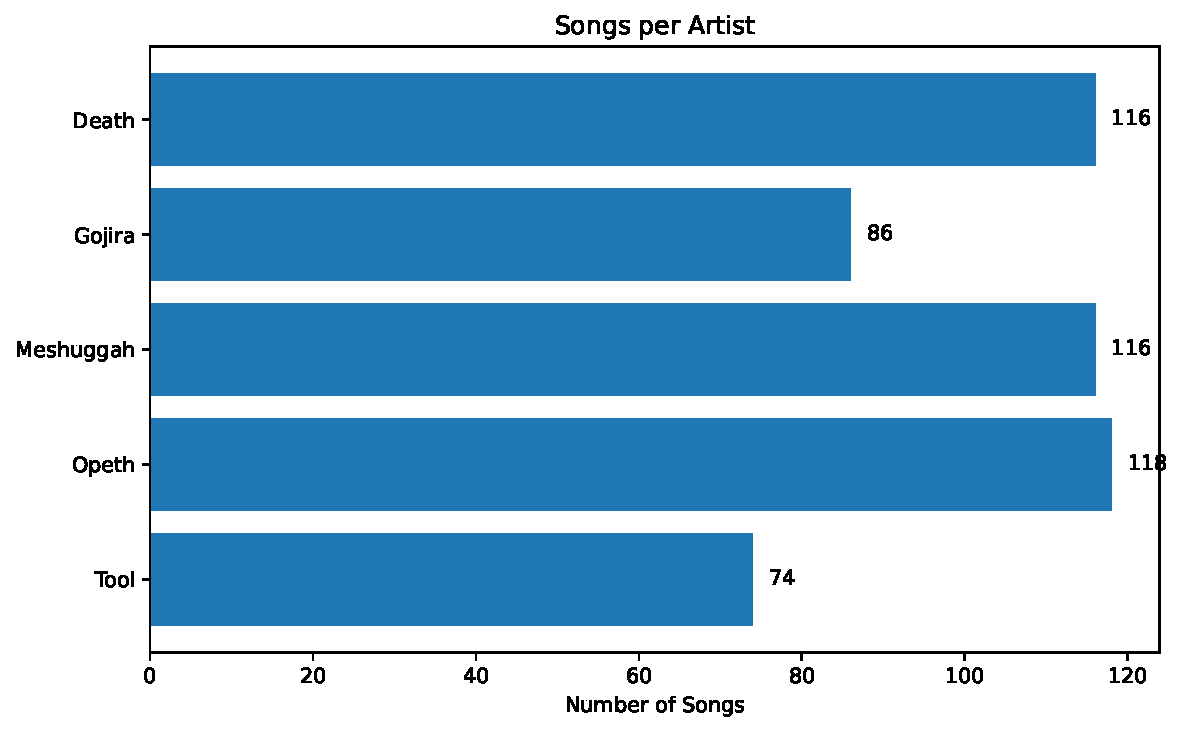
\includegraphics[width=\linewidth]{artist_distribution.pdf}
    \end{column}
  \end{columns}
\end{frame}

% ====================================================================
% ACT 1 -- TWO BASELINES, TWO FAILURES
% ====================================================================

% ---------- 3. Baseline 1: base model -> junk ----------
\begin{frame}{Baseline 1 --- pretrained \texttt{gemma-3n-E4B}: junk}
  \scriptsize\ttfamily\color{junk}\raggedright
  [User 0001]\ \ This is my band/artist page where you enter your range of audio, video --- preset unavailable for your region. To read lyrics from web, click back in your browser\ldots\par\vskip4pt
  [User 0001]\ \ [ame=http://youtube.com/\ldots]YouTube - Gero booyy[/video][/ame] \ldots you are wanting to post a video, hide it from devices. {\lt}b{\gt}Song Title{\lt}/b{\gt}\ \ 0 replies\ \ Added Friday, July 24, 2013\par\vskip4pt
  [User 0001]\ \ {\lt}b{\gt}GOJIRA!{\lt}/b{\gt}\ \ [User 0002]\ I'll be going down to the woods today\ \ Nooooooooo!!!!!\ \ [User 0003]\ In every dark place that this Gojira go..\par
  \normalfont\color{white}
  \take{The base model is a \emph{text predictor}, not a lyricist: it continues scraped forum/HTML noise. No prompt fixes this.}
\end{frame}

% ---------- 4. Baseline 2: instruct model -> fluent but collapsed ----------
\begin{frame}{Baseline 2 --- instruct \texttt{gemma-3n-E4B-it}: fluent, but one voice}
  \scriptsize\itshape\raggedright
  \textbf{\upshape Gojira:}\ \ \textbf{Beneath the obsidian} shroud, where silence breeds its dread reign\ldots\par
  \textbf{\upshape Mastodon:}\ \ \textbf{Beneath the obsidian} canopy, where fungal tides now creep and churn\ldots\par
  \textbf{\upshape Opeth:}\ \ \textbf{Beneath the} glacial shroud, a silence reigns supreme\ldots\par
  \textbf{\upshape Death:}\ \ Visceral rot descends on brittle bone\ldots\par
  \textbf{\upshape Tool:}\ \ The aperture narrows on a familiar hum\ldots\par
  \upshape\vskip4pt
  \footnotesize
  \begin{itemize}
    \item \textbf{Intra-artist:} all 10 Gojira samples open ``Beneath the obsidian/basalt shroud'' --- near-zero variance.
    \item \textbf{Inter-artist:} Gojira $\approx$ Mastodon $\approx$ Opeth all write ``Beneath the obsidian canopy.''
    \item \textcolor{accent}{Two baselines, two failures:}
      \begin{itemize}
        \item \textcolor{accent}{base $=$ incoherent junk}
        \item \textcolor{accent}{instruct $=$ coherent, but \emph{the same poem for every band}}
      \end{itemize}
      \textcolor{accent}{\textbf{Fluency is not style.}}
  \end{itemize}
\end{frame}

% ---------- 5. So we fine-tuned: method ----------
\begin{frame}{Fine-tune the pretrained base: one QLoRA adapter per artist}
  \begin{itemize}
    \item Base: \textbf{Gemma~3n~E4B} ($\sim$4B), QLoRA 4-bit NF4
    \item One \textbf{LoRA r8} adapter per artist (all linear layers)
    \item \textbf{Blend} two adapters in delta space (rank concatenation):
  \end{itemize}
  \vskip6pt
  \[
    A_{\text{blend}}=\begin{bmatrix}\alpha A_{1}\\[2pt](1-\alpha)A_{2}\end{bmatrix},\qquad
    B_{\text{blend}}=\begin{bmatrix}B_{1}&B_{2}\end{bmatrix}
  \]
  \take{$\alpha$ = weight of artist 1; endpoints recover the pure adapters exactly. Now: did it actually learn the artist?}
\end{frame}

% ====================================================================
% ACT 2 -- EVALUATION MACHINERY
% ====================================================================

% ---------- 6. The judge ----------
\begin{frame}{Evaluation is hard: generated lyrics have no label}
  \begin{columns}[c]
    \begin{column}{0.55\textwidth}
      \centering
      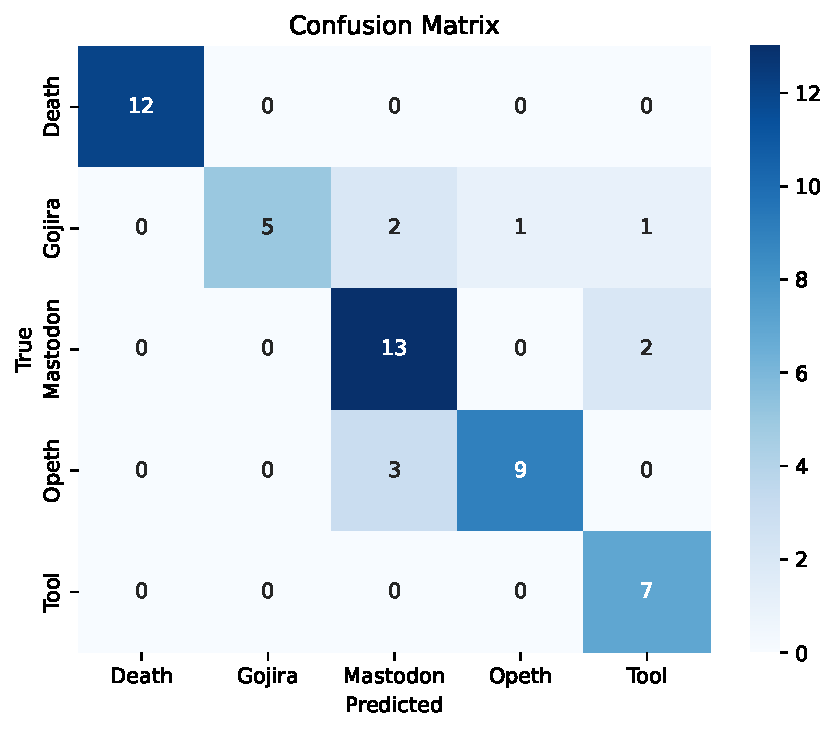
\includegraphics[height=0.62\textheight]{confusion_matrix.pdf}
    \end{column}
    \begin{column}{0.45\textwidth}
      \footnotesize
      \begin{itemize}
        \item \textbf{Problem:} no ground-truth label for generated lyrics.
        \item \textbf{Judge:} RoBERTa-base 5-way attribution classifier (acc \textbf{0.873}, macro-F1 \textbf{0.86}).
        \item \textbf{Score:} \metric{attribution} = P(target artist) --- high $\Rightarrow$ reads as the artist.
        \item \textbf{Caveat:} one machine judge --- a \textbf{sanity check, not ground truth} (can be gamed).
      \end{itemize}
      \take{No artist name in the prompt, yet attributed to its target $\Rightarrow$ the style is in the \emph{text}.}
    \end{column}
  \end{columns}
\end{frame}

% ---------- 6b. Adapter variants: DoRA + style-weighted loss ----------
\begin{frame}{Three ablations we run}
  \vfill
  \large
  \begin{itemize}\setlength{\itemsep}{16pt}
    \item \textbf{LoRA vs DoRA}\quad{\normalsize\color{junk}(weight-decomposed variant)}
    \item \textbf{LoRA rank ablation}\quad{\normalsize\color{junk}(r4 / r8 / r16)}
    \item \textbf{Plain LoRA vs style-weighted (SW) LoRA}\quad{\normalsize\color{junk}(TF-IDF-reweighted loss)}
  \end{itemize}
  \vfill
\end{frame}

% ---------- 7. Adapters attribute; baselines sink (+ correction 2) ----------
\begin{frame}{Adapters attribute; baselines collapse to a sink}
  \centering
  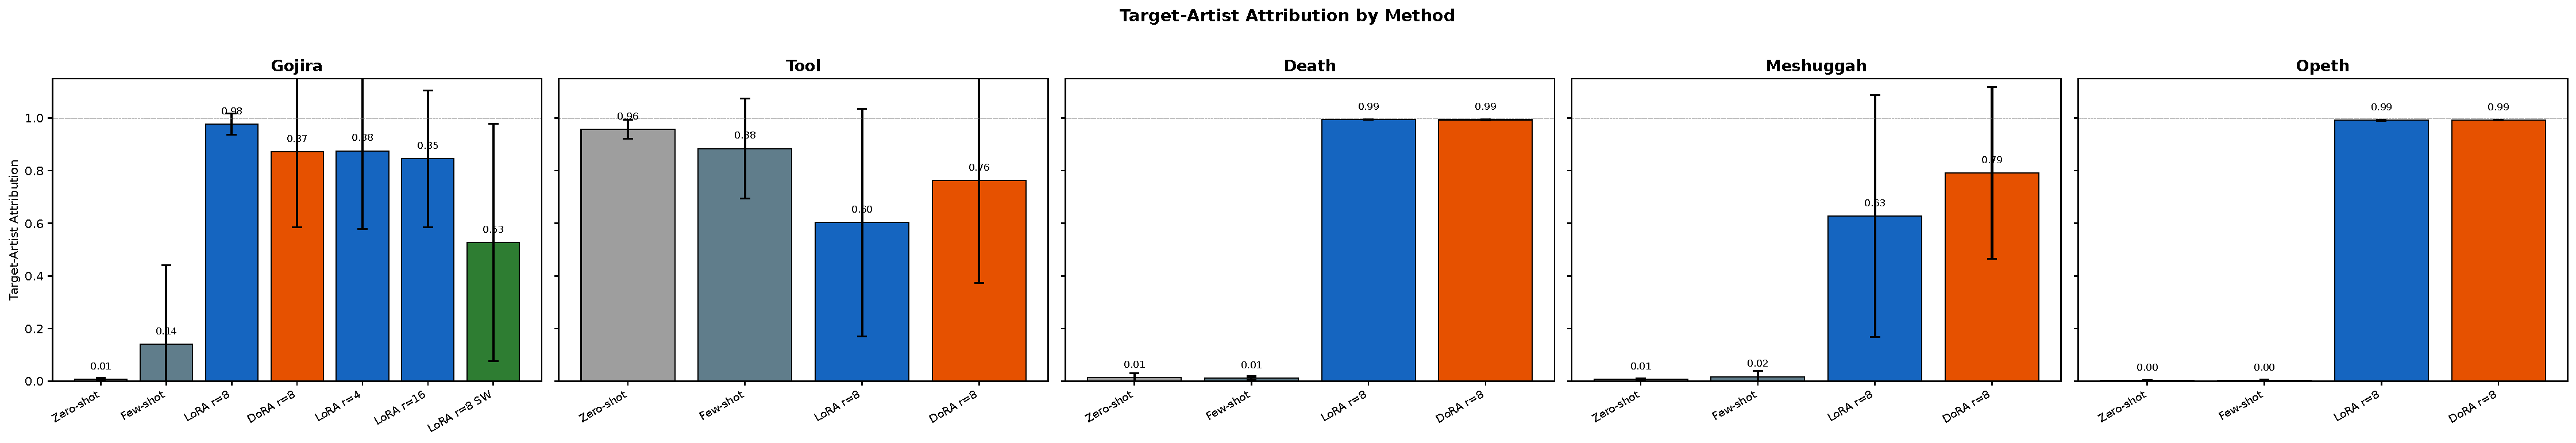
\includegraphics[width=0.98\linewidth]{method_comparison.pdf}
  \vskip6pt
  \begin{columns}[T]
    \begin{column}{0.56\textwidth}
      \footnotesize
      \begin{itemize}
        \item \textbf{No ``other'' class:} any out-of-distribution text is forced onto the \emph{nearest} real artist.
        \item \textbf{Not class imbalance:} majority class is Mastodon (154), yet neither sink is the majority:
          \begin{itemize}
            \item base $\rightarrow$ \textbf{Tool}
            \item instruct $\rightarrow$ \textbf{Opeth}
          \end{itemize}
          two different sinks.
      \end{itemize}
      \take{The sink isn't class imbalance, it's the classifier with no reject option. It only affects out-of-distribution text; adapters still attribute correctly.}
    \end{column}
    \begin{column}{0.44\textwidth}
      \centering\footnotesize
      \begin{tabular}{@{}lr@{}}
        \multicolumn{2}{c}{\textbf{Plain LoRA r8}}\\
        \toprule
        Target & \metric{attribution} \\
        \midrule
        Gojira   & 0.989 \\
        Death    & 0.903 \\
        Opeth    & 0.896 \\
        Mastodon & 0.873 \\
        Tool     & 0.689 \\
        \midrule
        base $\rightarrow$ Tool & $\approx$0.99 \\
        instruct $\rightarrow$ Opeth & $\approx$0.99 \\
        \bottomrule
      \end{tabular}
    \end{column}
  \end{columns}
\end{frame}

% ---------- 8. Ablation: rank ----------
\begin{frame}{Ablation: LoRA vs DoRA \& LoRA rank}
  \begin{columns}[c]
    \begin{column}{0.55\textwidth}
      \centering
      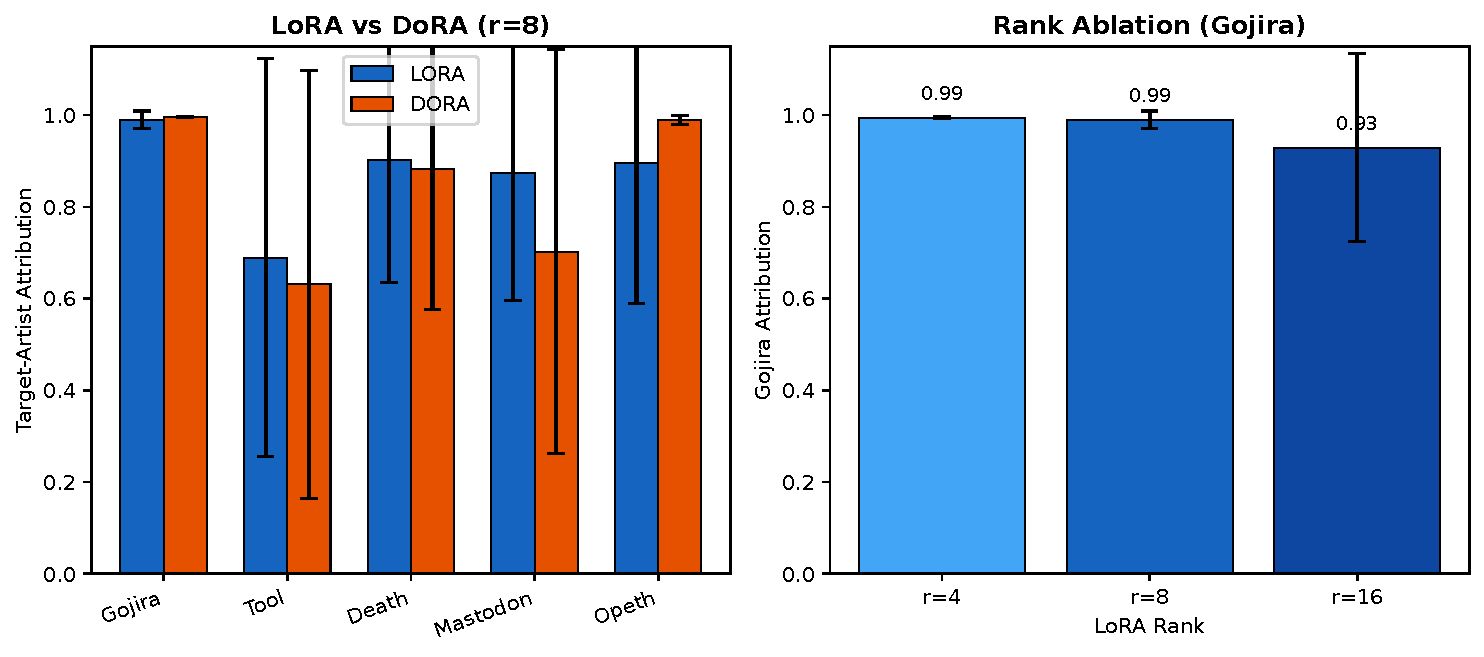
\includegraphics[width=\linewidth]{ablation.pdf}
    \end{column}
    \begin{column}{0.45\textwidth}
      \footnotesize
      \begin{tabular}{@{}lrrr@{}}
        \toprule
        Rank & Gojira & Tool & Mastodon \\
        \midrule
        r4  & \textbf{.994} & \textbf{.838} & \textbf{.987} \\
        r8  & .989 & .689 & .873 \\
        r16 & .929 & .755 & .824 \\
        \bottomrule
      \end{tabular}
      \take{r16 overfits; r4 matches/beats r8 on \metric{attribution}.}
    \end{column}
  \end{columns}
\end{frame}

% ---------- 9. Adapter lyrics showcase (flash & skip) ----------
\begin{frame}[t]{What the adapters actually write}
  \centerline{\footnotesize\color{junk}(plain LoRA r8 --- one sample per artist)}
  \vfill
  \scriptsize
  \begin{columns}[T]
    \begin{column}{0.33\textwidth}
      \textbf{Gojira}\par\itshape
      I took a boat across the ocean\\
      And I sail away, sailing home\\
      On an open sea that is so deep
    \end{column}
    \begin{column}{0.33\textwidth}
      \textbf{Death}\par\itshape
      In the dark of night\\
      The dead come forth from their graves\\
      A bloody ritual is being performed
    \end{column}
    \begin{column}{0.33\textwidth}
      \textbf{Opeth}\par\itshape
      I had a dream I was in the fall\\
      That everything would die away\\
      And when winter comes there is no more
    \end{column}
  \end{columns}
  \vskip8pt
  \begin{columns}[T]
    \begin{column}{0.33\textwidth}
      \textbf{Mastodon}\par\itshape
      The storm is coming down\\
      And sweeping through the trees\\
      Cleansing spirit, dispelling dreams
    \end{column}
    \begin{column}{0.33\textwidth}
      \textbf{Tool}\par\itshape
      My mind's on a different frequency\\
      So I might not see eye to eye with you\\
      I hear voices calling me away
    \end{column}
    \begin{column}{0.33\textwidth}
      \upshape\footnotesize\textcolor{accent}{Coherent, on-theme, no artist name in the prompt. So is the judge enough?}
    \end{column}
  \end{columns}
  \vfill
\end{frame}

% ====================================================================
% ACT 3 -- ONE NUMBER IS NOT ENOUGH
% ====================================================================

% ---------- 10. The metrics + their limits ----------
\begin{frame}{Beyond the judge: lexical metrics (and their limits)}
  \footnotesize
  \textbf{marker} = a characteristic token of an artist (top 40 per artist, stopwords dropped).
  \vskip4pt
  \begin{itemize}
    \item \metric{types} --- distinct markers $\Rightarrow$ \emph{breadth}
    \item \metric{occurrences} --- total markers $\Rightarrow$ \emph{repetition}
    \item \metric{distinct-2} --- unique bigrams $\Rightarrow$ \emph{degeneration} (looping)
  \end{itemize}
  \vskip4pt
  {\color{accent}Limitations --- no metric is neutral:}
  \begin{itemize}\footnotesize
    \item Token-level TF-IDF favors \textbf{concrete-noun} artists (Gojira: tree/star/forest) over \textbf{conversational} ones (Tool).
    \item Repetition can be real style (Tool's mantras) --- but \metric{occurrences} and the judge can't tell an artful motif from a degenerate loop.
  \end{itemize}
\end{frame}

% ---------- 11. CLIMAX: how the judge scores them ----------
\begin{frame}{How the judge scores them: higher score, worse lyrics}
  \vfill
  \begin{columns}[T]
    \begin{column}{0.5\textwidth}
      \centering\textbf{Plain Tool} --- score \textcolor{lo}{0.003}\par\vskip2pt
      \scriptsize\itshape
      \begin{tabular}{@{}l@{}}
      You know better than me\\
      What's what and why\\
      I might not be a prodigy\\
      But I can write a rhyme
      \end{tabular}
    \end{column}
    \begin{column}{0.5\textwidth}
      \centering\textbf{Style-weighted Tool} --- score \textcolor{hi}{0.996}\par\vskip2pt
      \scriptsize\itshape
      \begin{tabular}{@{}l@{}}
      Yeah, yeah\\
      Yeah, hey, hey\\
      Hey, hey, hey, hey\\
      Hey, hey, hey, hey\quad($\times$10)
      \end{tabular}
    \end{column}
  \end{columns}
  \vskip16pt
  \take{A degenerate ``hey'' loop \emph{beats} a coherent verse. Tool's gain is pure \metric{occurrences} (\metric{types} flat).}
  \vfill
\end{frame}

% ---------- 12. Three independent axes (all 5 artists) ----------
\begin{frame}{Four metrics, five artists --- they disagree}
  \centering\small
  \begin{tabular}{@{}lcccc@{}}
    \toprule
           & \metric{attribution} & \metric{types}/sample & \metric{occ.}/sample & \metric{distinct-2} \\
    Artist & (plain$\rightarrow$SW) & (plain$\rightarrow$SW) & (plain$\rightarrow$SW) & (plain$\rightarrow$SW) \\
    \midrule
    Gojira   & .99 $\rightarrow$ .67 & 1.6 $\rightarrow$ \textbf{5.7} & 1.9 $\rightarrow$ 11.9 & .96 $\rightarrow$ .71 \\
    Tool     & .69 $\rightarrow$ .90 & 2.5 $\rightarrow$ 3.3 & 3.1 $\rightarrow$ \textbf{28.5} & .88 $\rightarrow$ .74 \\
    Death    & .90 $\rightarrow$ .92 & 1.7 $\rightarrow$ 1.5 & 2.9 $\rightarrow$ 7.2 & .67 $\rightarrow$ .63 \\
    Mastodon & .87 $\rightarrow$ .87 & 2.0 $\rightarrow$ 3.3 & 2.7 $\rightarrow$ 4.9 & .90 $\rightarrow$ .70 \\
    Opeth    & .90 $\rightarrow$ .85 & 0.7 $\rightarrow$ 2.8 & 0.7 $\rightarrow$ 7.1 & .92 $\rightarrow$ .71 \\
    \bottomrule
  \end{tabular}
  \take{Breadth (\metric{types}) rises for Gojira/Opeth/Mastodon but not Tool/Death; \metric{occurrences} inflate everywhere; \metric{distinct-2} falls for all; \metric{attribution} moves both ways.}
\end{frame}

% ---------- 12b. Perplexity: clean diagonal, still disagrees on rank ----------
\begin{frame}{Perplexity --- a clean diagonal, yet it disagrees too}
  \centering
  \scriptsize
  \begin{tabular}{@{}lrrrrr@{}}
    \toprule
    & \multicolumn{5}{c}{held-out lyrics of}\\
    \cmidrule(l){2-6}
    adapter (r8) & Gojira & Tool & Death & Mastodon & Opeth \\
    \midrule
    base & 45.9 & 18.6 & 30.4 & 32.3 & 57.7 \\
    \midrule
    \multicolumn{6}{@{}l}{\itshape plain LoRA}\\
    Gojira   & \textbf{18.2} & 10.9 & 15.3 & 18.7 & 34.0 \\
    Tool     & 28.2 & \textbf{4.3} & 16.1 & 19.1 & 37.0 \\
    Death    & 70.3 & 24.6 & \textbf{4.5} & 49.5 & 105.6 \\
    Mastodon & 40.4 & 14.6 & 23.0 & \textbf{8.1} & 54.4 \\
    Opeth    & 29.0 & 12.2 & 16.5 & 20.7 & \textbf{9.5} \\
    \midrule
    \multicolumn{6}{@{}l}{\itshape style-weighted (SW)}\\
    Gojira   & \textbf{22.2} & 11.9 & 17.2 & 20.2 & 39.5 \\
    Tool     & 28.1 & \textbf{5.2} & 15.8 & 18.7 & 36.6 \\
    Death    & 49.8 & 19.1 & \textbf{6.6} & 36.8 & 71.3 \\
    Mastodon & 35.5 & 13.5 & 20.7 & \textbf{11.6} & 47.1 \\
    Opeth    & 35.1 & 13.4 & 19.3 & 22.7 & \textbf{16.9} \\
    \bottomrule
  \end{tabular}
  \take{Both blocks specialize (own-artist = column min, \textbf{bold}); but SW \emph{raises} every diagonal --- it buys artist vocabulary/\metric{attribution} at a likelihood cost. \metric{perplexity} rewards what SW penalizes.}
\end{frame}

% ====================================================================
% ACT 4 -- BLENDING + CLOSE
% ====================================================================

% ---------- 13. Blending crossover ----------
\begin{frame}{Blending: 50/50 weights $\neq$ 50/50 style}
  \centering
  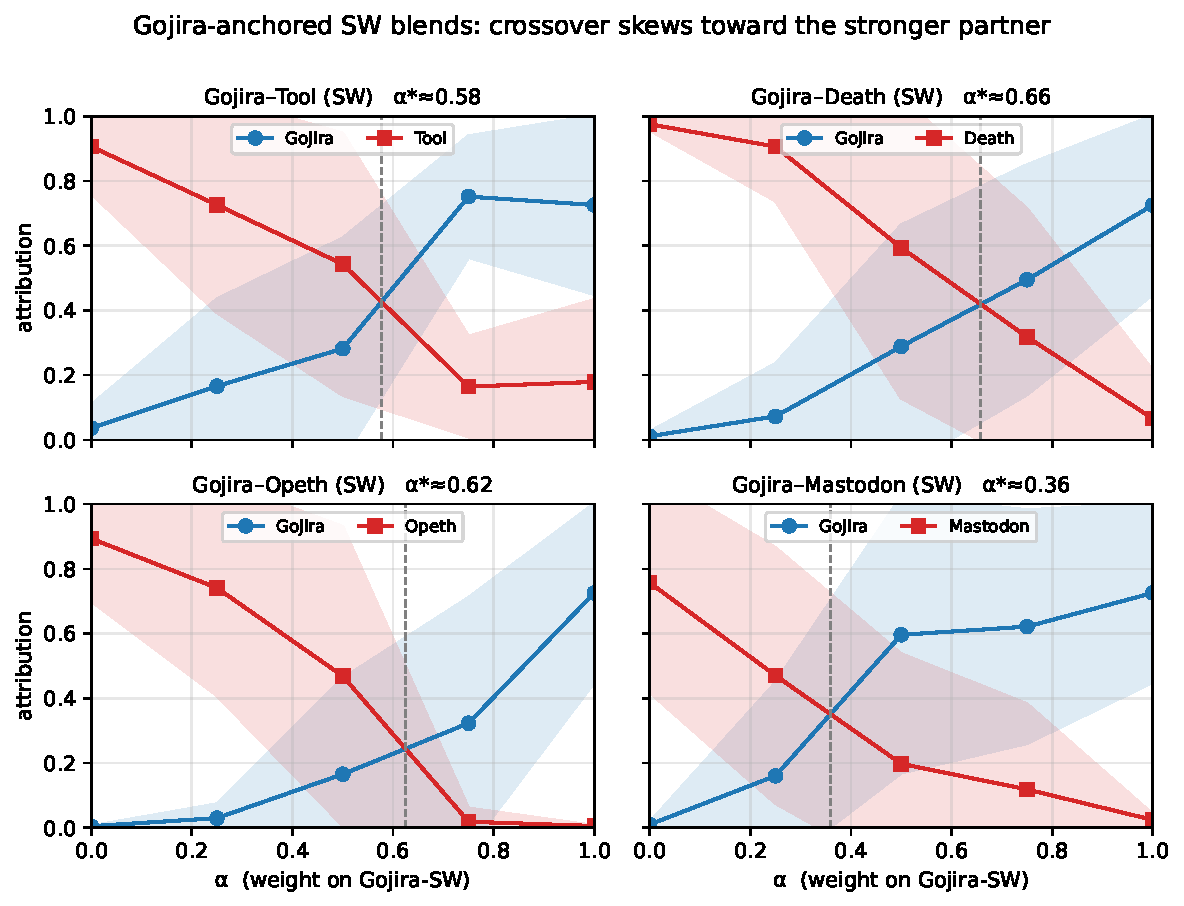
\includegraphics[width=0.95\linewidth,height=0.72\textheight,keepaspectratio]{blend_sw_gojira_partners.pdf}
  \take{\metric{attribution} (y) vs blend weight $\alpha$ (x). All four Gojira-SW blends cross over away from 0.5 (crossover at 0.47--0.65): the partner usually wins a 50/50 mix.}
\end{frame}

% ---------- 14a. Single Gojira (pure) ----------
\begin{frame}{Pure Gojira ($\alpha$=1.0) --- \textcolor{accent}{Gojira 1.00}}
  \scriptsize\itshape\raggedright
  \begin{columns}[T]
    \begin{column}{0.5\textwidth}
      No sense pretending to be innocent\\
      Don't even try, no reason now\\
      Kill this beast you call ``reason''\\
      Break the rules and break away the law\\[4pt]
      There is a vision coming alive in my mind\\
      Like bright fireflies flying free\\
      Awakening from the sleep I lay awake on the rock\\
      I understand it all\\[4pt]
      Create your own reality!\\
      You create yourself to become what you want to be\\
      And fight for better\\
      All alone against all of them
    \end{column}
    \begin{column}{0.5\textwidth}
      Enter your own realm --- open the door\\
      Leave all illusions behind --- step inside\\
      Set a course straight --- go along until the end\\
      Open your eyes embrace!\\[4pt]
      Enter your own realm --- open the door!\\
      Enter your own realm! ! !\\[4pt]
      This force that runs through you creates the world\\
      From matter and energy made --- structures fall apart!\\
      This force is running through me too --- create another\\
      Create --- create --- create --- another dimension!
    \end{column}
  \end{columns}
  \upshape\take{The anchor: coherent, cosmic/creation imagery (realm / force / matter and energy / dimension). Scored Gojira 1.00.}
\end{frame}

% ---------- 14b. Gojira + Tool ----------
\begin{frame}{Gojira + Tool ($\alpha$=0.5) --- \textcolor{accent}{Tool 0.99}}
  \scriptsize\itshape\raggedright
  \begin{columns}[T]
    \begin{column}{0.5\textwidth}
      I will rise and overcome\\
      Leave this cage for better\\[4pt]
      Fight back, fight back\\
      Don't you know I am alive?\\
      Fight back, fight back\\
      Don't you know I am alive?\\[4pt]
      Rise above the walls of hatred\\
      Learn to feel compassion\\
      Break the chains that bind us\\
      And understand why we must fight\\[4pt]
      Feel our wrath on your skin\\
      Feel our wrath on your skin\\
      Feel our wrath on your skin\\
      Feel our wrath on your skin
    \end{column}
    \begin{column}{0.5\textwidth}
      Don't you know I am alive?\\
      Don't you know I am alive?\\
      Don't you know I am alive?\\
      Don't you know I am alive?\\
      Don't you know I am alive?\\
      Don't you know I am alive?\\
      Don't you know I am alive?\\
      Don't you know I am alive?\\[4pt]
      Don't you know I am alive?\\
      Don't you know I am alive?\\
      Don't you know I am alive?\\
      Don't you know I am alive?
    \end{column}
  \end{columns}
  \upshape\vskip3pt\footnotesize
  \begin{itemize}\setlength{\itemsep}{1pt}
    \item \textbf{Gojira:} defiant uplift --- rise above hatred / break the chains / compassion
    \item \textbf{Tool:} the hypnotic 12$\times$ mantra
    \item \textcolor{accent}{\textbf{Verdict:} Tool 0.99 --- the loop, not imagery, wins}
  \end{itemize}
\end{frame}

% ---------- 14c. Gojira + Mastodon ----------
\begin{frame}{Gojira + Mastodon ($\alpha$=0.5) --- \textcolor{accent}{Tool 0.58 (a third artist)}}
  \scriptsize\itshape\raggedright
  \begin{columns}[T]
    \begin{column}{0.5\textwidth}
      I wonder if I'll ever learn to fly\\
      If it is right there in the sky\\
      If all the stars align and shine so bright\\
      Can you see them, baby? Can you count them?\\[4pt]
      And you said, ``It's good for your health''\\
      Good for your health\\
      Oh yeah, yeah, yeah\\
      Yeah, yeah, yeah\\[4pt]
      Get high, get high, get high\\
      Fly free, fly free, fly free\\
      Get high, get high, get high\\
      Fly free, fly free, fly free\\
      High above this beautiful world\\
      I can fly\\
      Fly through these open skies
    \end{column}
    \begin{column}{0.5\textwidth}
      In the night, the moon shines brightly on me\\
      I can feel her warmth come down to earth\\
      Bright eyes and teeth and golden skin\\
      She belongs to Mother Nature, the Earth\\
      Don't be afraid of falling down\\
      We all crawl from mud and bone\\
      Stand up tall and straight\\
      And ride that wave of life\\[4pt]
      Get high, get high, get high\\
      Fly free, fly free, fly free\\
      Get high, get high, get high\\
      Fly free, fly free, fly free\\
      Get high, get high, get high\\
      Fly free, fly free, fly free
    \end{column}
  \end{columns}
  \upshape\vskip3pt\footnotesize
  \begin{itemize}\setlength{\itemsep}{1pt}
    \item \textbf{Gojira:} earth/nature --- Mother Nature / mud and bone / wave of life
    \item \textbf{Mastodon:} astral flight --- fly free / high above / stars align
    \item \textcolor{accent}{\textbf{Verdict:} judge says \emph{Tool} (0.58) --- a third artist}
  \end{itemize}
\end{frame}

% ---------- 14d. Gojira + Opeth ----------
\begin{frame}{Gojira + Opeth ($\alpha$=0.5) --- \textcolor{accent}{Gojira 0.99 (anchor holds)}}
  \scriptsize\itshape\raggedright
  \begin{columns}[T]
    \begin{column}{0.5\textwidth}
      There's no escape\\
      I am trapped in a maze\\
      My soul is ablaze\\
      My heart is aching for what it knows\\
      Lost in space, lost on purpose\\
      Dream state I enter now\\[4pt]
      Open the door to another world\\
      Slip inside and let my spirit fly\\
      Take my hand and guide me there\\
      Help me find my way\\
      Into the night\\
      Inside you can hear nothing but silence\\
      And that voice crying out for love\\[4pt]
      Leave all behind, leave this old shell\\
      Leave alone, come back soon
    \end{column}
    \begin{column}{0.5\textwidth}
      Give us peace, give us time\\
      Set us free, release the spell\\
      Enter your mind\\
      Outside is wild, dangerous land\\
      We fight within the walls of our minds\\
      Stay with me awhile until dawn appears\\
      You are one of a kind\\
      Don't ever forget\\
      Never part again\\
      This is our destiny, always and forever more\ldots\\
      Until then we shall meet again in another realm\\
      Until then we shall meet again in another realm\\[4pt]
      No matter how long and hard you try\\
      In vain try to forget what came before\\
      How could you do this to me?\\
      I thought you cared, but now I know why
    \end{column}
  \end{columns}
  \upshape\vskip3pt\footnotesize
  \begin{itemize}\setlength{\itemsep}{1pt}
    \item \textbf{Gojira:} realm/another-world --- spirit fly / another realm / enter your mind
    \item \textbf{Opeth:} melancholic loss --- heart aching / ``voice crying out for love'' / ``I thought you cared''
    \item \textcolor{accent}{\textbf{Verdict:} anchor holds --- Gojira 0.99}
  \end{itemize}
\end{frame}

% ---------- 15. Gojira + Death ----------
\begin{frame}{Gojira + Death ($\alpha$=0.5) --- \textcolor{accent}{Mastodon 0.79 (a third artist)}}
  \scriptsize\itshape\raggedright
  \begin{columns}[T]
    \begin{column}{0.5\textwidth}
      Enter the land of darkness\\
      An ancient race now destroyed\\
      Lost in time and space forever\\
      Never to return\\[4pt]
      In the sky so clear you can see\\
      The flames burning bright below\\
      A giant dragon is breathing fire\\
      It grows ever stronger with each blow\\[4pt]
      Feel the heat flowing through your veins\\
      Fire at will, breathe and destroy\\
      Dragon is approaching fast\\
      Breath comes out as red hot steel\\
      Leave a trail of death behind you
    \end{column}
    \begin{column}{0.5\textwidth}
      Descend from the skies\\
      You've arrived\\
      Dragons of doom\\[3pt]
      Descend from the skies\\
      You've arrived\\
      Dragons of doom\\[3pt]
      Descend from the skies\\
      You've arrived\\
      Dragons of doom\\[3pt]
      Descend from the skies\\
      You've arrived\\
      Dragons of doom\quad\upshape\footnotesize($\times$7)
    \end{column}
  \end{columns}
  \upshape\vskip3pt\footnotesize
  \begin{itemize}\setlength{\itemsep}{1pt}
    \item \textbf{Gojira:} cosmic ruin --- ancient race destroyed / lost in time and space
    \item \textbf{Death:} violence --- breathe and destroy / red hot steel / trail of death
    \item \textcolor{accent}{\textbf{Verdict:} dragon/doom fantasy reads as \emph{Mastodon} (0.79), loops ``Dragons of doom'' 7$\times$}
  \end{itemize}
\end{frame}

% ---------- 15. Close + thesis ----------
\begin{frame}{Independent instrument, same verdict --- and the close}
  \begin{columns}[c]
    \begin{column}{0.55\textwidth}
      \centering
      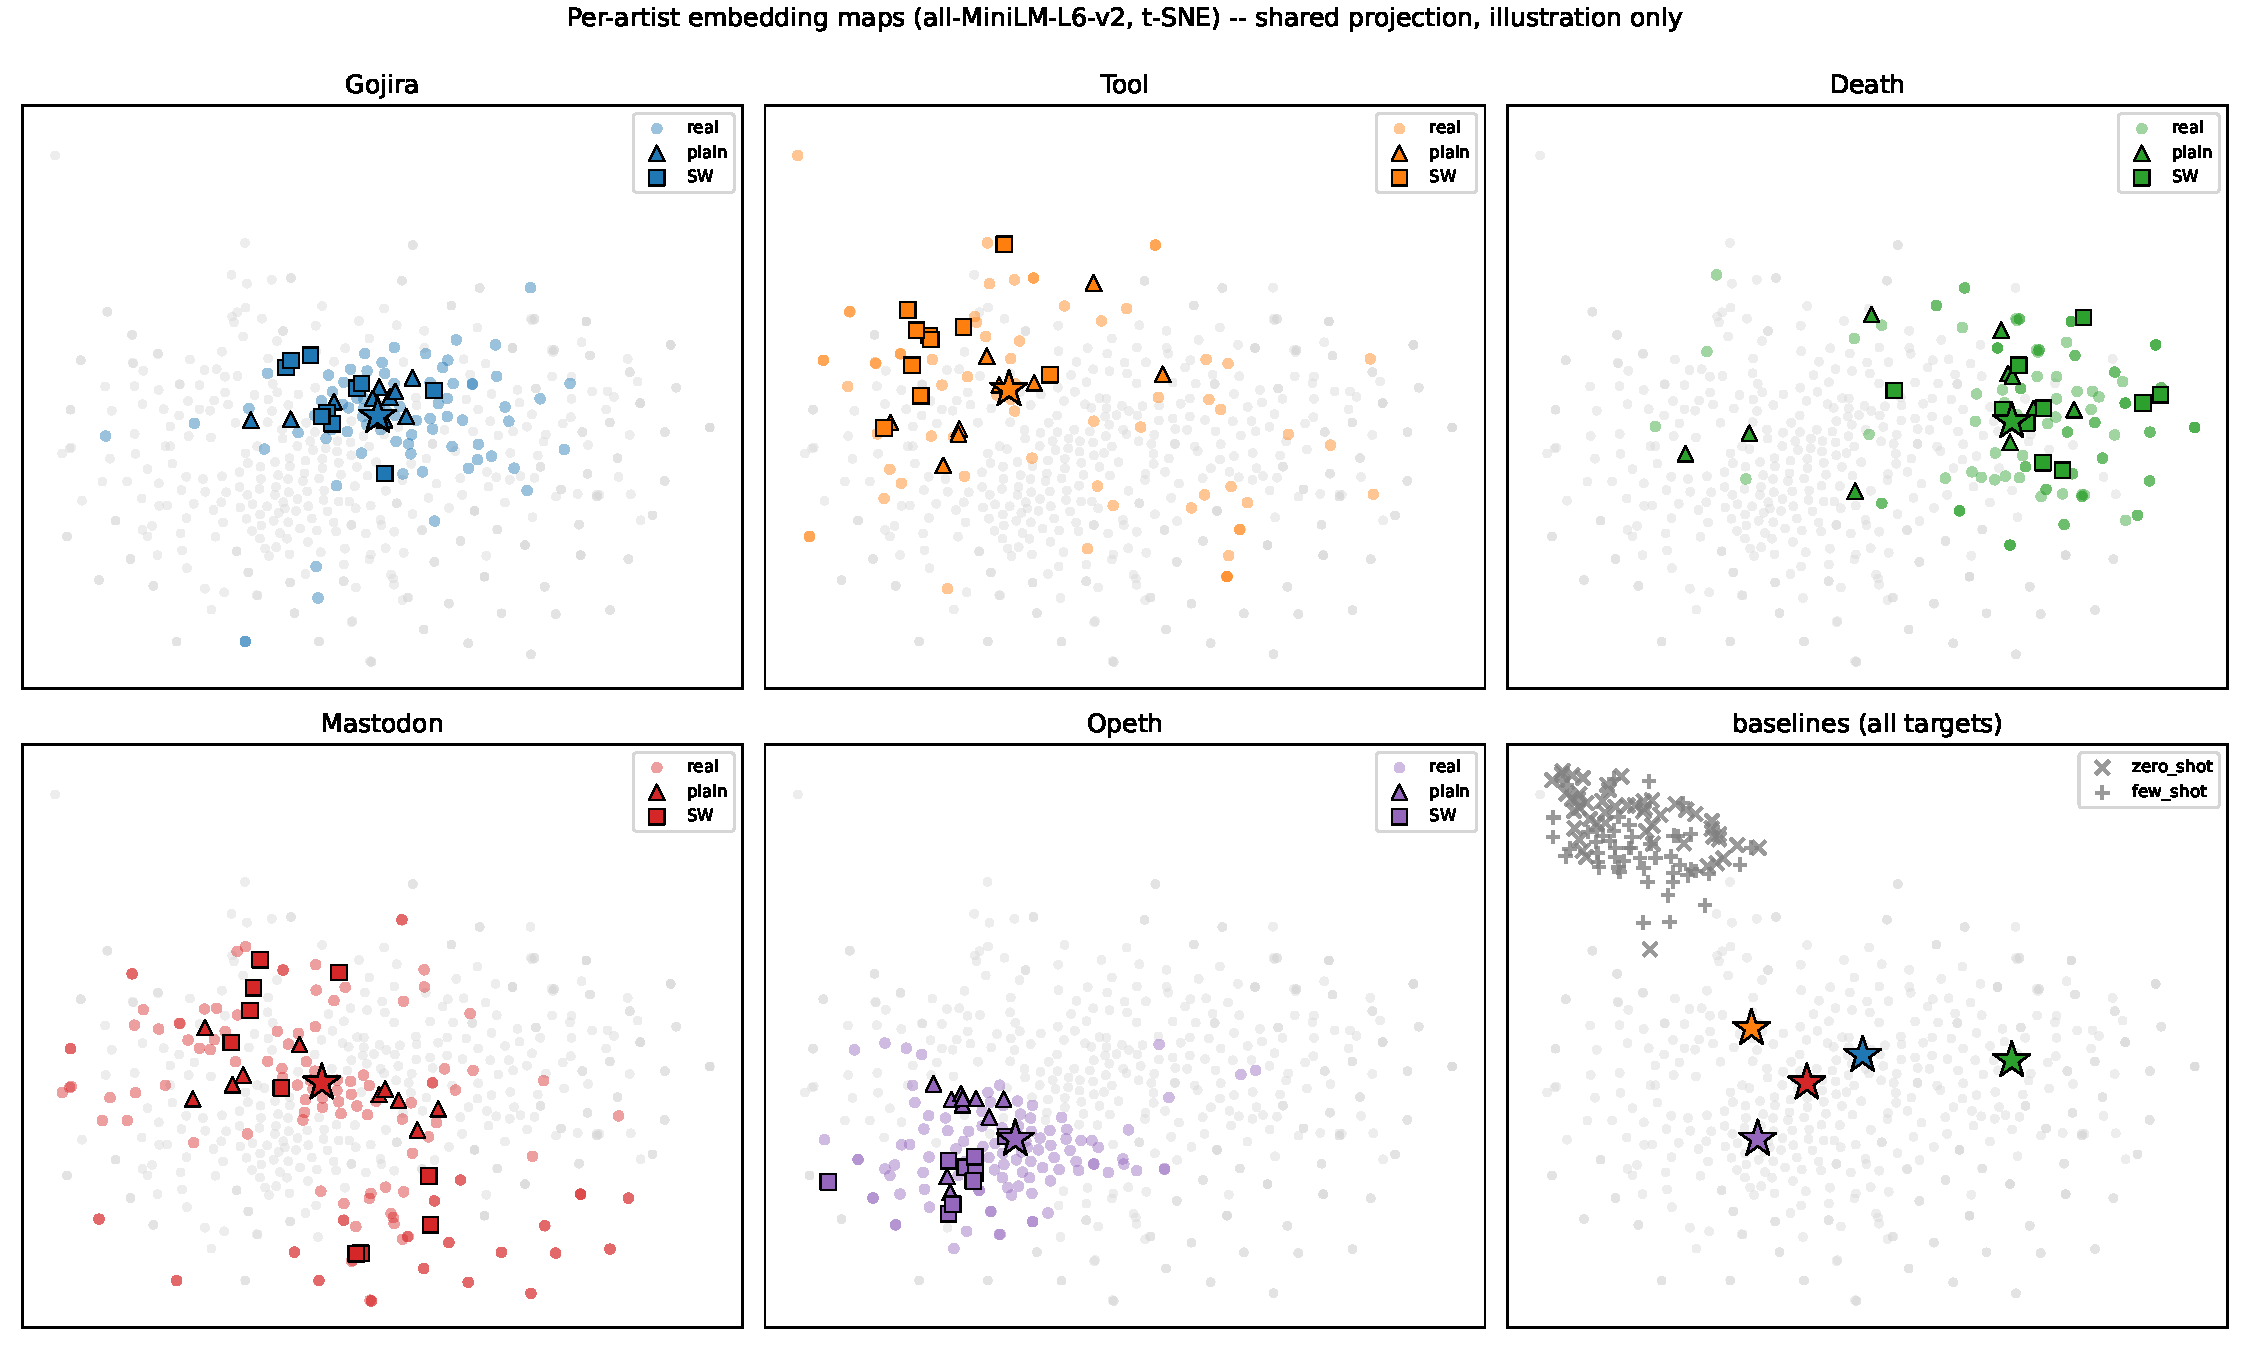
\includegraphics[height=0.6\textheight]{embedding_map_per_artist_tsne.pdf}
    \end{column}
    \begin{column}{0.45\textwidth}
      \footnotesize
      \begin{itemize}
        \item Adapters land on each artist's real-song cluster; base/instruct sit in OOD islands.
        \item No single metric captures a ``good'' generation --- \metric{attribution}, \metric{types}, and \metric{occurrences} pull in different directions.
        \item The most trustworthy measure is \textbf{human evaluation}, which one person alone cannot supply at scale.
      \end{itemize}
    \end{column}
  \end{columns}
  \vskip4pt
  \centering{\large\bfseries\textcolor{accent}{Style is not one number.}}
\end{frame}

\end{document}
